\section{Diseño de la arquitectura} % (fold)
\label{sec:diseno_de_la_arquitectura}

	\subsection{Diagrama de despliegue} % (fold)
	\label{sec:diagrama_de_despliegue}

		Un diagrama de despliegue muestra la configuración de los nodos de proceso y las instancias de componentes y objetos que residen en ellos. Los componentes representan unidades de código de ejecución. Los componentes que no existen como entidades de ejecución (porque se han compilado aparte) no aparecen en estos diagramas; deben aparecer en diagramas de componentes.

		\fcolorbox{negro}{gris}{\parbox{15cm}{Un Diagrama de Despliegue modela la arquitectura en tiempo de ejecución de un sistema. Esto muestra la configuración de los elementos de hardware (nodos) y muestra cómo los elementos y artefactos del software se trazan en esos nodos. Es decir se sitúa el software en el hardware que lo contiene. Cada Hardware se representa como un nodo.}}

		Los elementos usados por este tipo de diagrama son nodos (representados como un prisma), componentes (representados como una caja rectangular con dos protuberancias del lado izquierdo) y asociaciones.

		A continuación (Figura \ref{fig:despliegue}) podemos ver el diagrama de despliegue, que destaca por tener en un lado el equipo del cliente, y en el otro, el servidor de aplicación y de bases de datos.

			\begin{figure}[H]
			  \centering
			    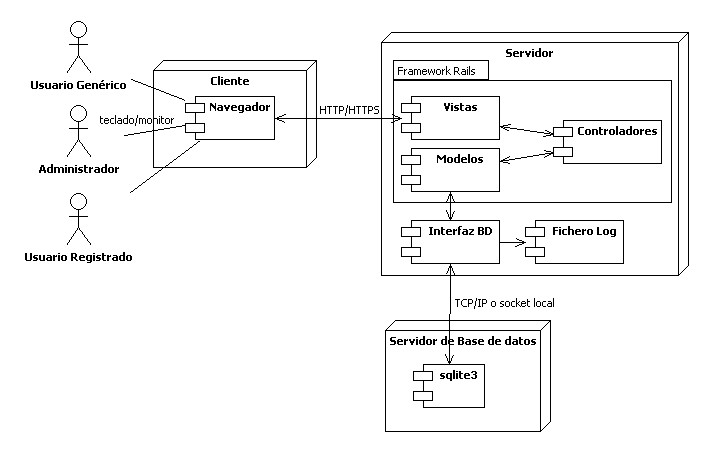
\includegraphics[width=16cm]{img/jpg/despliegue/despliegue.jpg}
			  \caption{Diagrama de Despliegue}
			  \label{fig:despliegue}
			\end{figure}


	% subsection diagrama_de_despliegue (end)

	\newpage
	\subsection{Diagrama de capas de diseño} % (fold)
	\label{sec:diagrama_de_capas_diseno}

		Como ya vimos en análisis, cualquier sistema grande se debe dividir en unidades más pequeñas, de modo que las personas puedan trabajar con una cantidad de información limitada, a la vez y de modo que los equipos de trabajo no interfieran con el trabajo de los otros. La gestión del modelo consiste en paquetes y relaciones de dependencia de los paquetes.

		Un paquete es, por tanto, una parte de un modelo. Además, cada parte de un modelo debe pertenecer a un paquete. El modelador puede asignar el contenido de un modelo a un conjunto de paquetes. Pero, para ser funcional, la asignación debe seguir un cierto principio racional, tal como funcionalidad común, implementación estrechamente relacionada, y un punto de vista común.

		En nuestro caso, vamos a agrupar los paquetes en base a tres capas. \textbf{La capa específica, la capa genérica y la capa Middleware. (Figura \ref{fig:dcapas}}. No es necesario que utilicemos la capa del sistema.

		En la primera, se hace mención a los paquetes propios de la aplicación, como son todos aquellos relacionados con las \textit{Actividades de los médicos, de los pacientes, de las fichas médicas, del administrador y de los usuarios genéricos.} Además, todos estos paquetes se dividen en subpaquetes, para agrupar una serie de actividades más específicas de cada uno de ellos. 

		Por su parte, en la segunda, se agrupan una serie de paquetes que pueden ser reutilizados en otras aplicaciones. En este proyecto son los relacionados con el \textit{registro de usuarios, algunas librerías javascript, la función autocompletar, la posibilidad de realizar paginación y todo lo relacionado con el multilenguaje.}

		En la tercera, vemos en más detalle las gemas utilizadas que dan sustento a las capas superiores.

		Una vez visto el diagrama general dividido en tres capas principales, con los subsistemas(paquetes) que contienen cada una de ellas, vamos a ver con más detalle los paquetes de la capa específica.

		En primer lugar, el paquete de \textit{Actividades de los médicos} (Figura \ref{fig:dcapas_medicos}), que está compuesto por \textit{Gestión del horario, del calendario, de los pacientes, de las plantillas, de las estadísticas y la administración.}

		A continuación tenemos los paquetes en los que están divididas las \textit{Actividades de los pacientes} (Figura \ref{fig:dcapas_pacientes}), que son \textit{la Gestión del calendario, de los médicos y de las fichas médicas.}

		Por último, vemos los paquetes que forman las \textit{Fichas médicas} (Figura \ref{fig:dcapas_fichas}). Éstos son \textit{Gestión de antecedentes, de informes, de tratamientos, de exploraciones, de pruebas y de observaciones}.

		\begin{figure}[H]
		  \centering
		    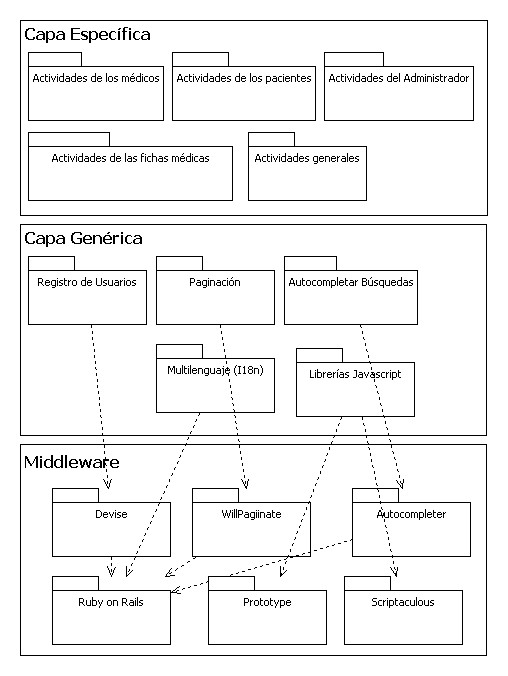
\includegraphics[width=16cm]{img/jpg/dcapas/capas.jpg}
		  \caption{Diagrama de Capas}
		  \label{fig:dcapas}
		\end{figure}



		\begin{figure}[H]
		  \centering
		    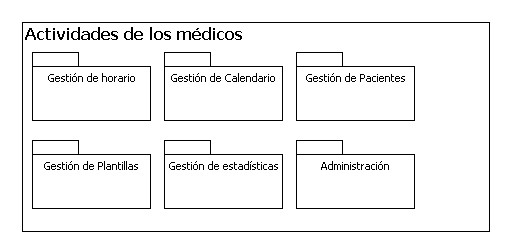
\includegraphics[width=12cm]{img/jpg/dcapas/Actividades_medicos.jpg}
		  \caption{Diagrama de Capas}
		  \label{fig:dcapas_medicos}
		\end{figure}

		\begin{figure}[H]
		  \centering
		    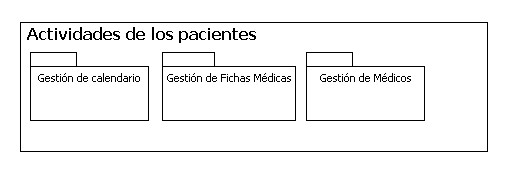
\includegraphics[width=12cm]{img/jpg/dcapas/Actividades_Pacientes.jpg}
		  \caption{Diagrama de Capas}
		  \label{fig:dcapas_pacientes}
		\end{figure}

		\begin{figure}[H]
		  \centering
		    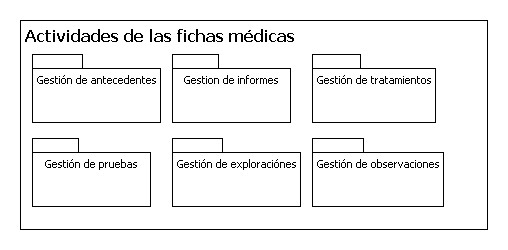
\includegraphics[width=12cm]{img/jpg/dcapas/fichas_medicas.jpg}
		  \caption{Diagrama de Capas}
		  \label{fig:dcapas_fichas}
		\end{figure}



	% subsection diagrama_de_capas (end)


% section diseño_de_la_arquitectura (end)